% vim: tw=80

\chapter{Jet Reconstruction}
\label{chap:jet_reconstruction}

In scattering processes with large momentum transfers, the outgoing partons
produce a collimated stream of particles when hadronizing. The cluster of these
particles are the experimental signatures of quarks and gluons in the detector
and are called \emph{jets}. Jets show up in the CMS detector as a localized
deposit of energy in the calorimeters accompanied by a large number of tracks in
the direction of the deposited energy. Jets are reconstructed using different
techniques based on the amount of information available. If the jets are
reconstructed from the energy clusters within the calorimeters, they are called
\emph{calorimeter jets}. If the jet reconstruction uses particle flow candidate
objects, these are called \emph{particle flow jets}. Later on, when talking
about jets in the physics analysis, we always refer to particle flow jets if not
stated otherwise.

\section{The Particle Flow Algorithm}
\label{sec:particle_flow_algorithm}

CMS uses the particle flow reconstruction
algorithm~\cite{CMS-PAS-PFT-09-001,CMS-PAS-PFT-10-001} to identify and
reconstruct particles in an event by combining information from all detector
subsystems. Due to its compact design inside the solenoid, the hadronic
calorimeter is not able to stop and measure all particles which reduces the
energy resolution. However taking into account the additional information of the
tracking system within the particle flow algorithm again improves the resolution
and leads to a comparable jet energy resolution as ATLAS. A key element in the
particle flow algorithm is the strong magnetic field of CMS which allows the
precise distinction between neutral and charged hadrons. 

The ingredients of the particle flow algorithm are the
tracks and vertices, reconstructed from hits in the tracking detectors, the
deposited energy in the electromagnetic and hadronic calorimeters and the tracks
in the muon system. The reconstructed particles are then classified as muons,
electrons, photons, charged hadrons or neutral hadrons. The combination of all
subdetectors yields an optimal determination of their momentum, energy and type.

The tracks are found using the Combinatorial Track Finder (CTF)
algorithm~\cite{Adam:2005cg} employed by CMS. Based on these tracks, the primary
vertices in an event are identified. The electromagnetic and hadronic
calorimeters are divided into a grid of cells based on the detector granularity
to identify calorimeter cluster seeds. If there are seeds with an energy
exceeding a certain threshold, they are used in an iterative merging algorithm
to form particle flow clusters. The different elements of the detector
information are then linked together into particle flow building blocks based on
the geometry and \chisq fits. At first muons, which can be well identified
using the tracks in the muon detector, are reonstructed using the building
blocks connected to the muon system. Blocks connecting the inner
tracking system with the ECAL clusters are used to identify electrons.
Similarly charged hadrons are identified using links between the
tracking system and the remaining calorimeter clusters. Only neutral objects
which leave no traces in the tracking system. ECAL clusters are
interpreted as photon candidates, while the remaining HCAL clusters are assumed
to be deposits of neutral hadrons. To avoid any kind of double-counting of
energy, all particle flow building blocks of succesfully reconstructed particle
candidates are removed and the energy of the calorimeter clusters is recalculated.

Finally a set of so called particle flow candidates is yielded consisting of
well identified particles, which profit from the improved resolution gained by
the inclusion of the tracking information. This collection of particles is then
used to reconstruct the jets and further physical objects.

\section{Jet Algorithms}
\label{sec:jet_algorithms}

The information of the clustered stream of particles, known as jets, provide the
link between the short-scale physics and our final-state observations. There
are many different algorithms available which cluster jets from a set of input
objects. Many of them were found to have their specific problems and today,
both \CMS and \ATLAS rely on the \antikt and inclusive \kt jet algorithms which proved to be very
robust and both are collinear and infrared safe, see Section~\ref{sec:coll_safety}.
They are sequential recombination algorithms and combine the input objects based on a
distance measure in Minkowski space.

\subsection{Collinear and Infrared Safety}
\label{sec:coll_safety}

Hard partons undergo many collinear splittings in the fragmentation process.
Additionally there are always emissions of soft particles in QCD-like events,
caused by non-perturbative and perturbative effects. The reconstructed jets
should be insensitive to all these effects. Additionally, fixed-order pQCD
calculations are associated with diverged tree-level matrix elements and the
corresponding loop matrix level elements. While these divergences cancel for
infared and collinear safe jets, this is not guaranteed for jet algorithms not
fullfilling the infrared and collinear safety requirements. Figure~\ref{fig:infrared_safety}
shows the effect of a collinear splitting and of additional soft particles on
the results of an unsafe jet algorithm. Most of the cone based jet algorithms which cluster
elements based on a constant distance in the $\eta-\phi$ space are affected by
the mentioned issues leading to the popularity of the modern sequential recombination
algorithms which are used in almost all of todays jet-based analyses.

\begin{figure}[htb]
    \centering
    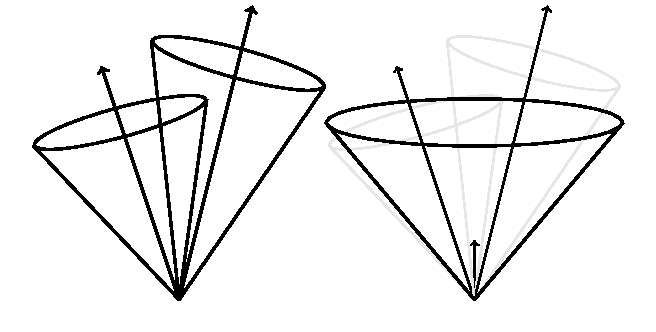
\includegraphics[width=0.5\textwidth]{figures/drawings/infrared_safety/jetinfrared.pdf}\hfill
    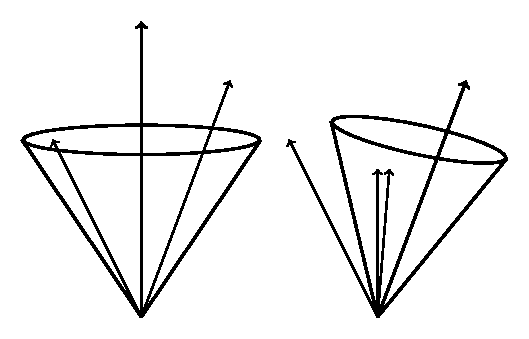
\includegraphics[width=0.45\textwidth]{figures/drawings/infrared_safety/jetcollinear.pdf}
    \caption{The left figure shows an illustration of an in infrared unsafe jet
        algorithm. By adding an additional soft particle the jet configurations
        change. The right sketch shows an quasi-collinear splitting which again leads,
        for an collinear unsafe jet algorithm, to a changed jet clustering result.}
    \label{fig:infrared_safety}
\end{figure}

\subsection{Generalized \kt Jet Algorithm}

The most popular sequential recombination algorithms are the \kt jet
algorithms which cluster jets based on a jet size parameter $R$ and an
additional parameter $p$ introducing a dependence on the transverse momentum of
the input objects. The pair-wise algorithm uses a list of input objects like stable
particles or particle flow candidates. 

At first the distances $d_{ij}$ between two particles and the distances to the
beam  $d_{iB}$ are calculated based on the rapidity difference $\Delta y_{ij}$
and the azimuthal angle $\Delta \phi_{ij}$ betwen two particles $i$ and $j$.

\begin{align} 
    d_{ij} &= \min(p_{\mathrm{T}i}^{2p},p_{\mathrm{T}j}^{2p})\frac{\Delta R_{ij}^2}{R^2}\\
    d_{i\mathrm{B}} &= k_{\mathrm{T}i}^{2p}
\end{align} 

with the angular distance

\begin{align}
    \Delta R_{ij}^2 &= (\Delta y_{ij})^2 + (\Delta \phi_{ij})^2
\end{align} 

If distance $d_{ij}$ is smaller than the distances to the beam line, the two
particles $i$ and $j$ are merged into a new particle $k$ which replaces the
particles $i$ and $j$ in the input list. These steps are repeated until all
particles are clustered into jets. Since the distance measures are defined in
Minkowski space, the shapes in the $\eta-\phi$ plane are not circular but
irregular, see Figure~\ref{fig:jet_shapes}. Based on the parameter $p$, there
are three important \kt based algorithms with distinct properties

\begin{figure}[htb]
    \centering
    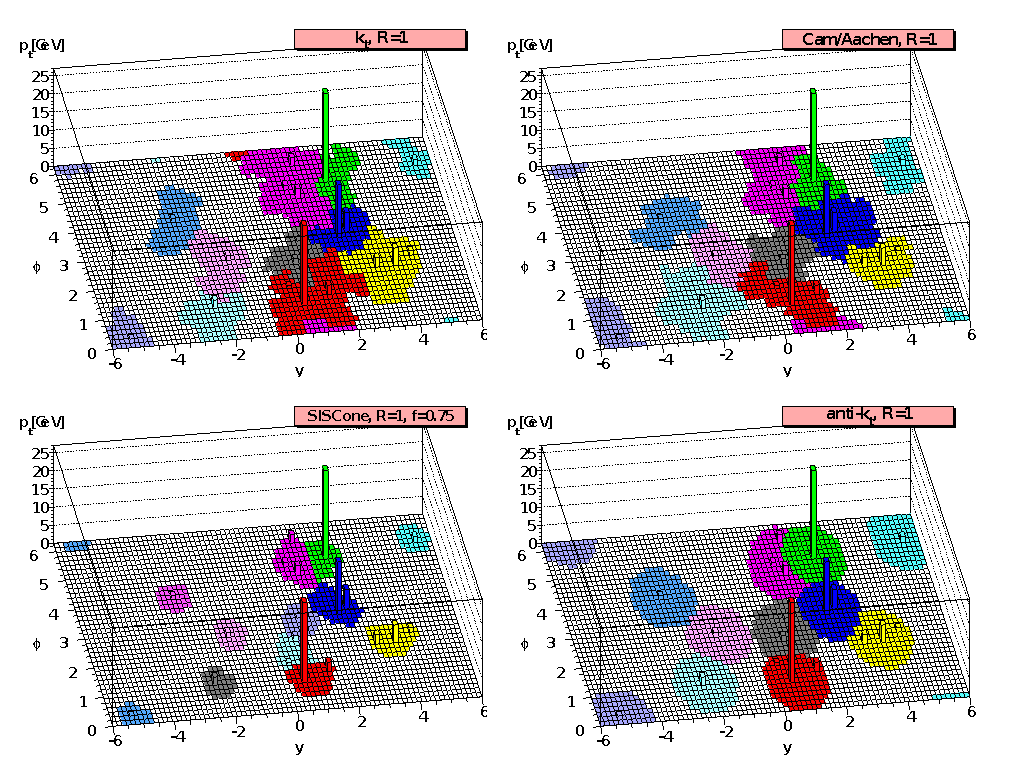
\includegraphics[width=0.8\textwidth]{figures/jet_reconstruction/jet_shapes.pdf}
    \caption{The obtained jet areas for the described \kt based algorithm
        and the cone-based SISCone algorithm~\cite{Salam:2009jx}. The \antikt
        algorithm yields circular shapes for hard jets while soft jets are crescent
        shaped.}
    \label{fig:jet_shapes}
\end{figure}

\begin{itemize}
    \item The \textbf{Inclusive \kt algorithm ($p=1$)} is based on a \ptsq
        distance measure which attempts to approximately describe the inversion
        of the QCD branching process.
    \item The \textbf{Cambridge-Aachen algorithm ($p=0$)} is only based on the
        spatial separation of the objects and does not rely on the energy of
        the input objects. Similarly to the inclusive \kt algorithm its jets
        have an irregular shape. This jet algorithm is in particular interesting
        for jet substructure studies.
    \item The \textbf{Anti-\kt algorithm ($p=-1$)} favours clustering hard input
        objects resulting in fairly circular jet shapes for hard jets, while
        soft jets are crescent-shaped if they are close to a hard jet~\cite{Cacciari:2008gp}.
\end{itemize}

\subsection{Jet Area}

The jet area describes the space in the $\eta$-$\phi$ plane covered by a jet
object. While cone-based jet algorithms yield a $\pi R^2$ size area, the area
for sequential based jet areas needs to be determined for each jet. A large
number of infinitely soft particles, so-called ghost particles, are evenly
distributed in the event and the area of a jet $A_j$ is assumed to be propoprtinal to the
number of ghost particles clustered into the jet $j$. The jet area is
especially important in the context of pile-up mitigation, which makes use of
the median pile-up and underlying event \pt density $\rho$ in the event 
\begin{equation}
    \rho = \text{median} \frac{\pt^j}{A_j}
\end{equation}
describing the median energy deposition per unit area.

\section{Jet Energy Corrections}

A detailed understanding of the jet energy scale and the jet transverse momentum
resolution is important to draw conclusions about the properties of quarks and
gluon produced in high-energy prcesses. On experimental side, there are multiple
effects causing the reconstructed jet energy to not correspond to the true jet
energy like electronic noise, pile-up and underlying event effects, but also
non-linearities in the calorimeter response and numerous further small effects.
The jet reconstruction and definition itself also introduces effects due to the
fragmentation model, initial state- and final state radiation which can cause
out-of-cone effects.

The jet energy corrections (JEC) relate the measured jet energy to the
corresponding true particle jet energy. CMS uses a factoriced correction approach
consisting of multiple corrections steps based on each other. The total
correction factor to be applied on an uncorrected jet is

\begin{equation}
    \pt^{\mathrm{corr}} = c_{\mathrm{res}} (\eta, \pt') \cdot c_{\mathrm{mc}}
    (\eta \pt'') \cdot c_{\mathrm{pileup}}(\eta, \rho, A_j, \pt^{\mathrm{raw}}) \cdot \pt^{\mathrm{raw}} 
\end{equation}

where $\pt^{\mathrm{raw}}$ is the transverse momentum of the uncorrected jet,
$\pt'$ the transverse momentum after applying the pile-up correction and $\pt''$
the transverse momentum after the additional correction $c_\mathrm{MC}$ of
relative and absolute effects from MC studies. Finally a correction for residual
effects derived from data $c_{\mathrm{res}}$ is applied to yield the corrected
jet transverse momentum $\pt^{\mathrm{corr}}$.

\subsection{Pile-up Corrections}

The first step removes the effects of pile-up contamination. Additional soft proton-proton
interactions produce particles being clustered into the jets originating from
the hard interaction. This additional amount of energy needs to be subtracted by
the pile-up correction. The applied correction is based on the jet area method
by using the pile-up density $\rho$ in the event and the jet area $A$. The raw
jet energy is then corrected by a factor proportional to the pile-up density and
the jet area.

\subsection{MC Corrections}

Based on a QCD data samples the jet energy scale is further corrected. The
momentum of a reconstructed jet can differ from a generated particle jet due to
additional out-of-cone effects or detector ineffiencies, which are modelled
using the detector simulation. The inverse response of the reconstructed jet to
a generated jet is applied as correction to remove these effects.

\subsection{Residual Data Corrections}

Additional effects which can not be reliably estimated in a Monte Carlo
simulation are corrected for using data-driven methods. This correction step is
only applied on data. The relative residual corrections are based on
well-balanced dijet events in which a forward probe jet is calibrated using a
tag jet in the well understood barrel region. The last correction step is the
absolute residual correction in which reconstructed Z bosons balanced to a jet
are used to calibrate the jet energy using the very precisely reconstructed Z
boson.

\todo{MET/CHF/JETBild?}
